



\chapter{Smart Grid Cyber attacks}
%Overview of cyber attacks
%\section{Threat Actors}
%Threat actors
%- Threat actor Categories
%  - MitM
%  - MotS
%- Threat actor Capabilities

%\section{Types of Cyber Attacks}
%Cyber Attacks
%- Cyber Attack Categories
%  - (D)DoS
%  - FDI
%  - Time Delay Attack
%  - Malware





%\chapter{Cyber Attacks on the Smart Grid}









The \acrfull{sg} is a complex system delivering electrical power to a society more dependant on electricity then ever, given the transition from traditional sources of energy to electrical energy on areas like agriculture, industrial production, heating, and more recently, transportation.
The transition of the electrical grid from the classic \acrlong{pg} to the \acrlong{sg} exposed, as previously described, the \acrlong{ci} of the power grid to attacks from remote locations via the Internet. 


\section{Attack via time protocols}

Computer systems reachable\footnote{Systems could ultimately be targeted utilising USB sticks, if not accessible from the Internet.} from the outside world,  are potential targets of Cyber attacks. The eventual recoveries of the initial Cyber Attacks was followed up by defence actions, resulting in more advanced attack techniques, has evolved to a continuous battle of control between attackers and defenders. \\


\subsubsection{Threat Actor  Types}
There are numerous Threat Actors of various skill levels, from so-called "Script Kiddies" to professionals, aiming to get unauthorised access to systems, for fun, fame, or for more serious reasons, like terrorism or financial gain. 

\begin{itemize}
    \item The \textbf{Internal attacker} has privileged access to, at least parts of, the internal infrastructure of the target, enabling the ability to take malicious actions not available to non-internal attackers.
    \item The \textbf{External attacker} is limited to attacking the targeted infrastructure from the outside, typically through network connections.
    \item The \textbf{Traffic Injector attacker} adds network packages to the benign traffic of the networks of the target, in order to produce the desired effects on the state and operation of the targeted infrastructure. 
    \item The \textbf{\acrshort{mitm} attacker} interrupts the communication between the two parties A and B, impersonating as B to A and vice-versa.
    \item The  \textbf{\acrshort{mots} attacker} are able to eavesdrop on communications, without any privileged access to enable the direct modification of any data transmitted.
\end{itemize}



The various types of attackers possesses various malicious action capabilities, which they may use in order to attack their intended target in numerous ways.


%\subsection{Time  Protocol Threats}










\subsection{Examples of Cyber attacks}
As described in \cite{sundararajan2019survey}, a number of security incidents targets the \acrshort{sg} specifically, like the 2015 BlackEnergy3 attack on the Ukranian  Power Grid, the StuxNet worm of 2010, as well as the watering-hole remote access trojan attack of 2014. 
Any online \acrshort{sg} infrastructure containing vulnerabilities, is equally inflicted by attacks not specifically targeting \acrfull{sg} like the WannaCry ransomware cryptoworm of 2017, targeting the EternalBlue vulnerability of unpatched windows computers.







%\subsubsection{Time Synchronisation attacks}
\section{Cyber Attacks targeting Smart Grid}

The two-way communication lines of the\acrlong{sg} systems opens the possibilities of communication between the networks of energy distributors and the networks of consumers, serving purposes as automatic measurement of energy consumption, as well as dynamic adaption of energy production according to variations in demand for energy over the hours of the day.
The transition from networks managed by closed communication channels to networks communicating over IP-based networks, exposes\acrlong{sg} networks to Cyber attack vulnerabilities.
Malicious threat actors having privileged access to the infrastructure, is able to perform various kinds of internal attacks.\\

Traditionally, anyone aiming to attack the \acrlong{pg} infrastructure, was obliged to get physical access to the premises, from which the infrastructure in question was controlled. Following the transition to the online \acrshort{sg}, the network connecting the grid to the outside might be utilised in order to execute any Cyber attack requiring internal privileged access from the outside.


\subsection{External Attacks}
External attacks is characterised by malicious actors attacking the infrastructure from the outside, without having the privileged access required in order to target internal system vulnerabilities.


\subsection{Internal Attacks}
The distinction between external and internal attacks, is the level of access required in order to perform the attack in question.

\subsubsection{Man on The Side (MoTS) Attack}
The \acrfull{mots} attack is a type of attack requiring minimal privileges and system access in order to be successfully executed.




\begin{figure}
    \centering {
    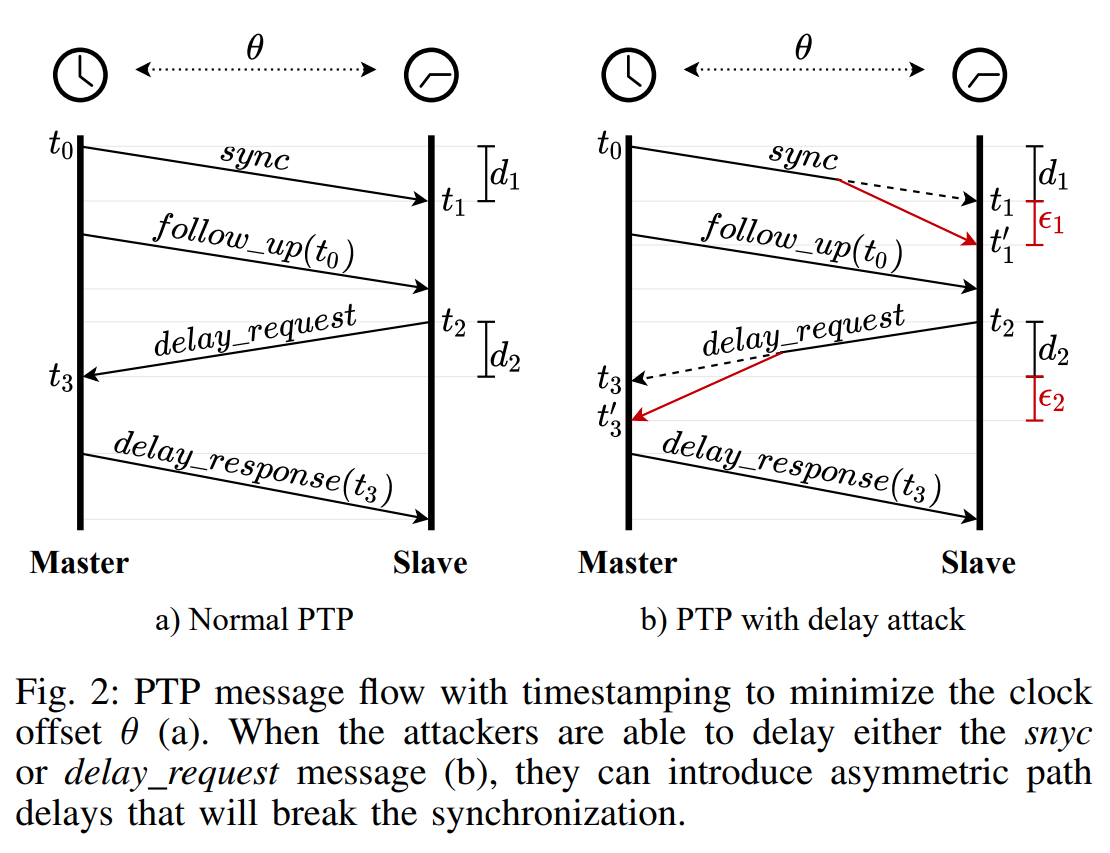
\includegraphics[ width=0.9\textwidth]{figures/PTP-delay attack.png}
    \caption[PTP Sync: Normal sync vs. sync under PTP Delay attack]{As presented in \cite{finkenzeller2022feasible}, figure 2. Comparison of PTP delay attack synchronisation with normal PTP synchronisation.}
    \label{fig:PTP-DelayAttack}
  }
\end{figure}  



\section{PTP delay Attacks} \label{sec:PTP-delay}
Several attacks which targets the \acrlong{ptp}  utilises vulnerabilities in the PTP, as explained by \cite{finkenzeller2022feasible}:


Based on the equations related to the regular \acrshort{ptp} synchronisation, in \cite{finkenzeller2022feasible} stated as:



\begin{equation} \label{eq:5-t1}
t_1 = t_0 + \theta + d_1 
\end{equation}

\begin{equation} \label{eq:5-t3}
t_3 = t_2 - \theta + d_2 
\end{equation}

\begin{equation}   \label{eq:5-d1}
d_1 = d_2 = d  
\end{equation}

%\textbf{Bla bla }Equation \ref{eq:5-t1}

\begin{equation}  \label{eq:5-offset}
\theta = \frac{(t_1 - t_0) - (t_3 - t_2)}{2}
\end{equation}


\begin{equation}  \label{eq:5-d}
d  = \frac{(t_1 - t_0) + (t_3 - t_2)}{2}
\end{equation}


The PTP delay attack uses the following equations:

\begin{equation}
    t'_1 = t_0 + \theta + d_1 + \epsilon_1
\end{equation}


\begin{equation}
    t'_3 = t_2 - \theta + d_2 + \epsilon_2
\end{equation}


Using the equation \ref{eq:5-d}, we arrive at  the following equations:



\begin{equation}  \label{eq:5-dtheta}
\theta' = \frac{(t_1 - t_0) - (t_3 - t_2)}{2} - \frac{\epsilon_1 - \epsilon_2}{2}
\end{equation}

\begin{equation}  \label{eq:5-d-delay}
d' = \frac{(t_1 - t_0) - (t_3 - t_2)}{2} - \frac{\epsilon_1 + \epsilon_2}{2}
\end{equation}

and accordingly:
\begin{equation}
    \theta' = \theta - \frac{\epsilon_1 - \epsilon_2}{2} 
\end{equation}

and \\

\begin{equation}
    d' = d - \frac{\epsilon_1 + \epsilon_2}{2} 
\end{equation}


For the attack, \citeauthor{finkenzeller2022feasible} further describes, the attacker has the option to set the desired (erroneous) clock offset value at will, as well as being able to control the offset direction. choosing vvalues of $\epsilon_1$ and  $\epsilon_1$ as $\epsilon_1 < \epsilon_2$  for setting the slave behind, whereas the reverse is true for the case of  $\epsilon_1 > \epsilon_2$. \\ 

Thus the \acrshort{ptp} delay is a realistic attack. Some of the various flavors of the attack should be obtainable for an attacker having limited access to the Target of the attack, like a \acrfull{mots} attacker.